\clearpage
\chapter*{Annexure C: Criteria 3 Supporting Documents}
\phantomsection
\addcontentsline{toc}{chapter}{Annexure C: Criteria 3 Supporting Documents}
\label{app:crtieria-3}



% \clearpage
% \phantomsection
% \chapter*{Annexure C: Criteria 3 Supporting Documents}
% \addcontentsline{toc}{chapter}{Annexure C: Criteria 3 Supporting Documents}
% \label{app:crtieria-3}

This section provides supporting annexures required for the Criterion 3: Curriculum and Learning Process.

% \setcounter{section}{0}
% \renewcommand{\thesection}{C.\arabic{section}}

\setcounter{section}{0}
\renewcommand{\thesection}{C.\arabic{section}}
\renewcommand{\theHsection}{annexC.\arabic{section}}


\phantomsection
\section{Intake 2K25 WP No. 30, 72nd ACM}
\label{app:criteria3-intake-2k25-wp30}
The BE Software Engineering (BESE) curriculum at SEECS, NUST, was revised to align the program with the Pakistan Engineering Council (PEC) Engineering Education Guidelines for implementing the Higher Education Commission’s Undergraduate Education Policy (UEP-2024). The revision responds to the mandatory inclusion of specified general education courses in undergraduate engineering programs from Fall 2025 and aims to maintain compliance with the updated credit-hour requirements while preserving the sequence of core Software Engineering courses.

The revised curriculum introduces Fehm-e-Quran-I (1 credit hour) in the first semester and Fehm-e-Quran-II (1 credit hour) in the second semester. Applications of ICT (2+1 credit hours) is also introduced in the first semester. In addition, Pakistan Studies (2 credit hours) is reintroduced as a compulsory course in the fourth semester, replacing the earlier arrangement in which Ideology and Constitution of Pakistan was offered in the first semester. These changes address the prescribed general education requirements under HEC UEP-2024 and the PEC framework.

To maintain an appropriate distribution of credit hours, several existing courses have been relocated between semesters. Occupational Health and Safety and Sociology Elective-II have been moved to the eighth semester, while Expository Writing and Discrete Mathematics have been repositioned within the curriculum. Selected mathematical courses have also been rescheduled. These adjustments help satisfy the minimum requirement of 15 credit hours per semester, where applicable, and the maximum limit of 21 credit hours, without disrupting the progression of core technical courses.

The revision also removes Engineering Drawing and Workshop Practice, which were part of the earlier common first-year engineering structure but are no longer required under the updated PEC curriculum for Software Engineering. Their removal supports compliance with the prescribed maximum of 140 credit hours and creates greater scope for domain-specific and industry-relevant learning. Furthermore, the number of core engineering elective courses has increased from five to six, with corresponding adjustments to elective credit-hour allocations. The semester-wise placement of electives remains flexible, allowing courses to be offered with different credit-hour configurations, as specified in the revised scheme.

Overall, the 2025 revision incorporates the requirements of HEC UEP-2024 and the updated PEC framework while refining course sequencing, elective provision, and credit-hour distribution. The proposal was approved by the Faculty Board of Studies (FBS) on 8 July 2025 and endorsed by the University Curriculum Review Committee (UCRC) on 28 August 2025. The revised unified BE Software program at SEECS and MCS was recommended for implementation from the Fall 2025 batch.
\includefullannexure{appendices/criterion_3/Annex-1-WP-30-72-ACM.pdf}

\clearpage
\phantomsection
\section{Intake 2K24 WP No. 20, 69th ACM}
\label{app:criteria-3_intake-2k24-wp20}

The BE Software Engineering (BESE) curriculum at SEECS, NUST, was revised to align the program with the Pakistan Engineering Council (PEC) Engineering Education Guidelines for the adoption of the Higher Education Commission’s Undergraduate Education Policy (UEP-2023). The revision was proposed in accordance with the PEC framework issued in September 2023 and recommended for implementation in the Fall 2024 intake. The primary objective was to ensure regulatory compliance while maintaining the prescribed credit-hour limits and a balanced distribution of courses across semesters. The revision introduced changes to the humanities component of the curriculum, particularly the knowledge area WK-7: Engineering in Society. In the first semester, the existing English (2 credit hours) course was replaced with Functional English (3 credit hours) to meet the revised requirements. Similarly, Communication Skills (2 credit hours) in the second semester was replaced with Expository Writing (3 credit hours). These changes strengthened the formal English and writing components in accordance with the PEC guidelines. To accommodate the increased credit hours without exceeding the prescribed semester limits, the curriculum was reorganized while retaining a maximum of 18 credit hours per semester where applicable.

The revision also updated the Pakistan-related studies requirement. Pakistan Studies (2 credit hours) in the first semester was replaced with Ideology and Constitution of Pakistan (2 credit hours). In addition, Occupational Health and Safety (1 credit hour) was moved from the first to the second semester, while Islamic Studies (2 credit hours) was shifted from the second to the fourth semester. The revised curriculum provides Ethics (2 credit hours) alongside Islamic Studies in the fourth semester for non-Muslim students, in accordance with the proposed framework. Further adjustments were made to the distribution of humanities and elective courses. Sociology Elective-I was moved from the fourth semester to the fifth semester, where it replaced Technical and Business Writing (2 credit hours), which was removed from the curriculum. These changes reorganized the non-technical course component while preserving the overall structure of the eight-semester degree program.

The revision largely retained the existing technical and core Software Engineering courses, including programming, database systems, data structures and algorithms, software design and architecture, software quality engineering, cloud computing, information security, software project management, and the final-year design project. The changes therefore focused primarily on compliance with the revised PEC requirements and the redistribution of selected humanities and supporting courses rather than a fundamental restructuring of the technical curriculum.

Overall, the revision updated the BESE curriculum to incorporate the requirements associated with HEC UEP-2023 and the PEC framework, strengthened the English and writing components, revised the Pakistan studies requirement, and improved the sequencing of selected courses. The proposal was endorsed by the University Curriculum Review Committee (UCRC) on 23 July 2024 and approved by the Faculty Board of Studies (FBS), as recorded in Working Paper No. 20 for the 69th Academic Council Meeting held on 6 August 2024. The revised curriculum was recommended for implementation in the BE Software Engineering program at SEECS and MCS from the Fall 2024 batch.

\includefullannexure{appendices/criterion_3/Annex-2-WP-20-69-ACM-1-6.pdf}

\clearpage
\phantomsection
\section{Intake 2K19 WP No. 30, 64th ACM}
\label{app:criteria-3_intake-2K19-wp30}
 The program was based on the Pakistan Engineering Council’s 2020 curriculum, which was approved in August 2021. The reason for this revision was a NUST policy change to the Final Year Project (FYP). Previously the FYP carried 3 credit hours in each of the seventh and eighth semesters, but NUST had reduced the seventh-semester load to 2 credit hours and raised the eighth-semester load to 4. This redistribution left some semesters below the minimum regular credit-hour load, so the curriculum needed small adjustments to make up the difference.

The first change is simply the FYP credit split itself: SE-498 (Final Year Project I) now carries 2 credit hours in semester 7, and SE-499 (Final Year Project II) carries 4 credit hours in semester 8. This applies to all ongoing batches, meaning the Fall 2019 intake and everything after it. The remaining changes differ depending on the intake. For the Fall 2019 and Fall 2020 batches, the paper adds a new two-credit Social Science Elective, ECO-130 (Engineering Economics), to the eighth semester. This brings that semester to 12 credit hours and the whole program to 135 credit hours, made up of 110 teaching and 25 lab hours.

For the Fall 2021 and later batches, no new course was added. Instead, two electives swap places. Engineering Elective IV (Data Warehousing and Data Mining), a 3-1 course, moves from semester 7 to semester 8, while MDEE-II (Internet of Things), a 3-0 course, moves from semester 8 to semester 7. This rebalances the workload so both semesters meet the minimum. The program total for these batches is 131 plus X credit hours, where X represents the lab component of certain electives that varies depending on the course chosen. The full revised semester-wise course lists for both groups appear in Annex I and Annex II.

On the practical side, the paper states that no extra instructors or classrooms are required. The proposal was approved by the Faculty Board of Studies on 16 November 2022 and endorsed by the University Curriculum Review Committee on 16 December 2022. The paper itself says the changes take effect from Fall 2022, while the Academics Directorate recommends implementation from Spring 2023 and asks the Academic Council to make the final decision. The stated aim is to keep the BESE program aligned with the PEC’s revised curriculum while improving the quality of final year projects in line with academic and industry needs. Everything else in the existing curriculum remains unchanged.

\includefullannexure{appendices/criterion_3/Annex-3-WP-30-64-ACM.pdf}

\clearpage
\refstepcounter{section}
\phantomsection \label{app:criteria-3_Course Outline with Knowledge Group Head's Signature}
\addcontentsline{toc}{section}{\protect\numberline{\thesection}Course Outline Vetted by Knowledge Group Head}

% ---- Page 1: shrunk, shifted down, heading above it ----
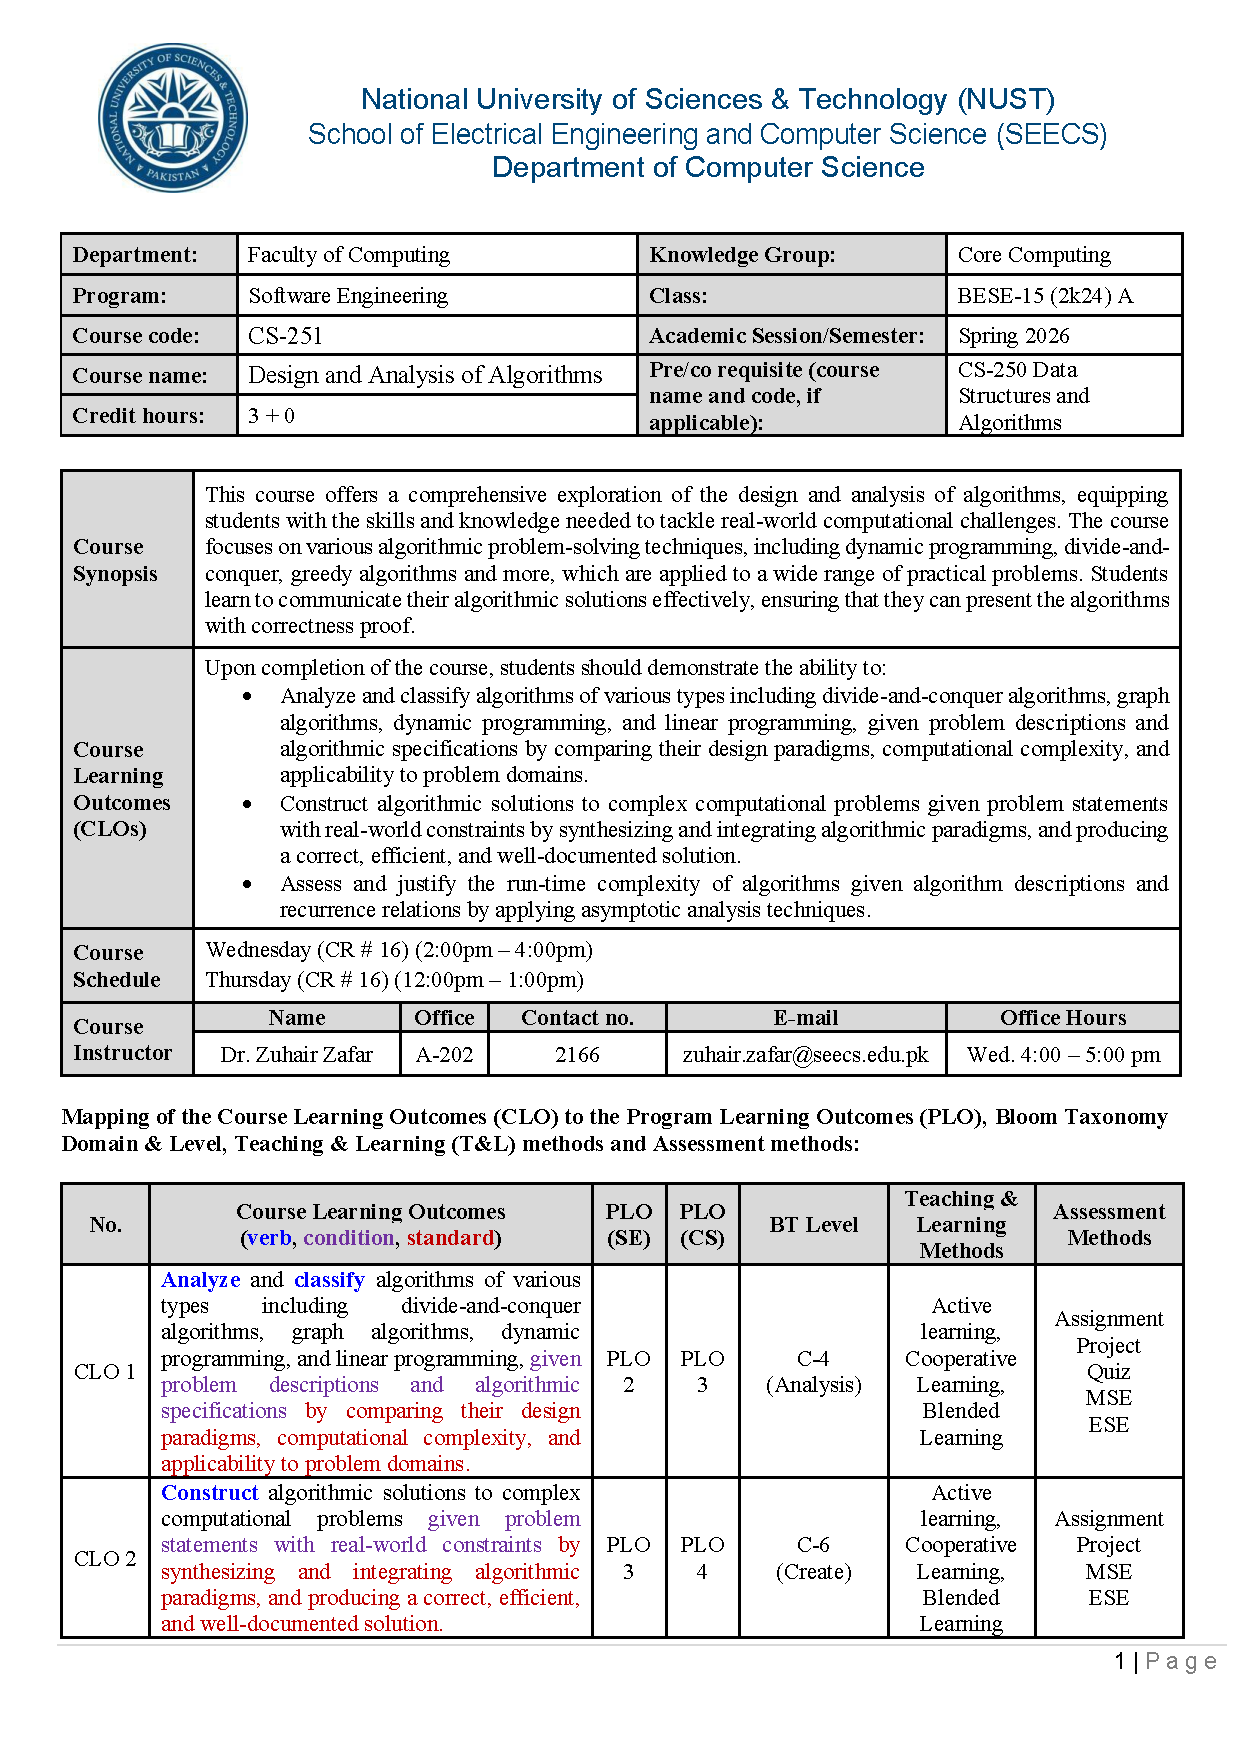
\includepdf[
  pages={1},
  scale=0.85,
  offset=0 -1.5cm,
  pagecommand={\thispagestyle{plain}%
    \noindent{\Large\bfseries\thesection\quad Course Outline Vetted by Knowledge Group Head}}
]{appendices/criterion_3/Annex-4-Course_outline_CS-251 Design and Analysis of Algorithms Spring 2026.pdf}

% ---- Pages 2 to end: unchanged, at full size ----
\includepdf[
  pages={2-},
  pagecommand={\thispagestyle{plain}}
]{appendices/criterion_3/Annex-4-Course_outline_CS-251 Design and Analysis of Algorithms Spring 2026.pdf}

\clearpage
%\section{PLO Attainment Transcript}

\refstepcounter{section}
\phantomsection 
\label{app:criteria-3_PLO Attainment Transcript}
\addcontentsline{toc}{section}{\protect\numberline{\thesection}PLO Attainment Transcript}
\begin{landscape}
% ---- Page 1: shrunk, shifted down, heading above it ----
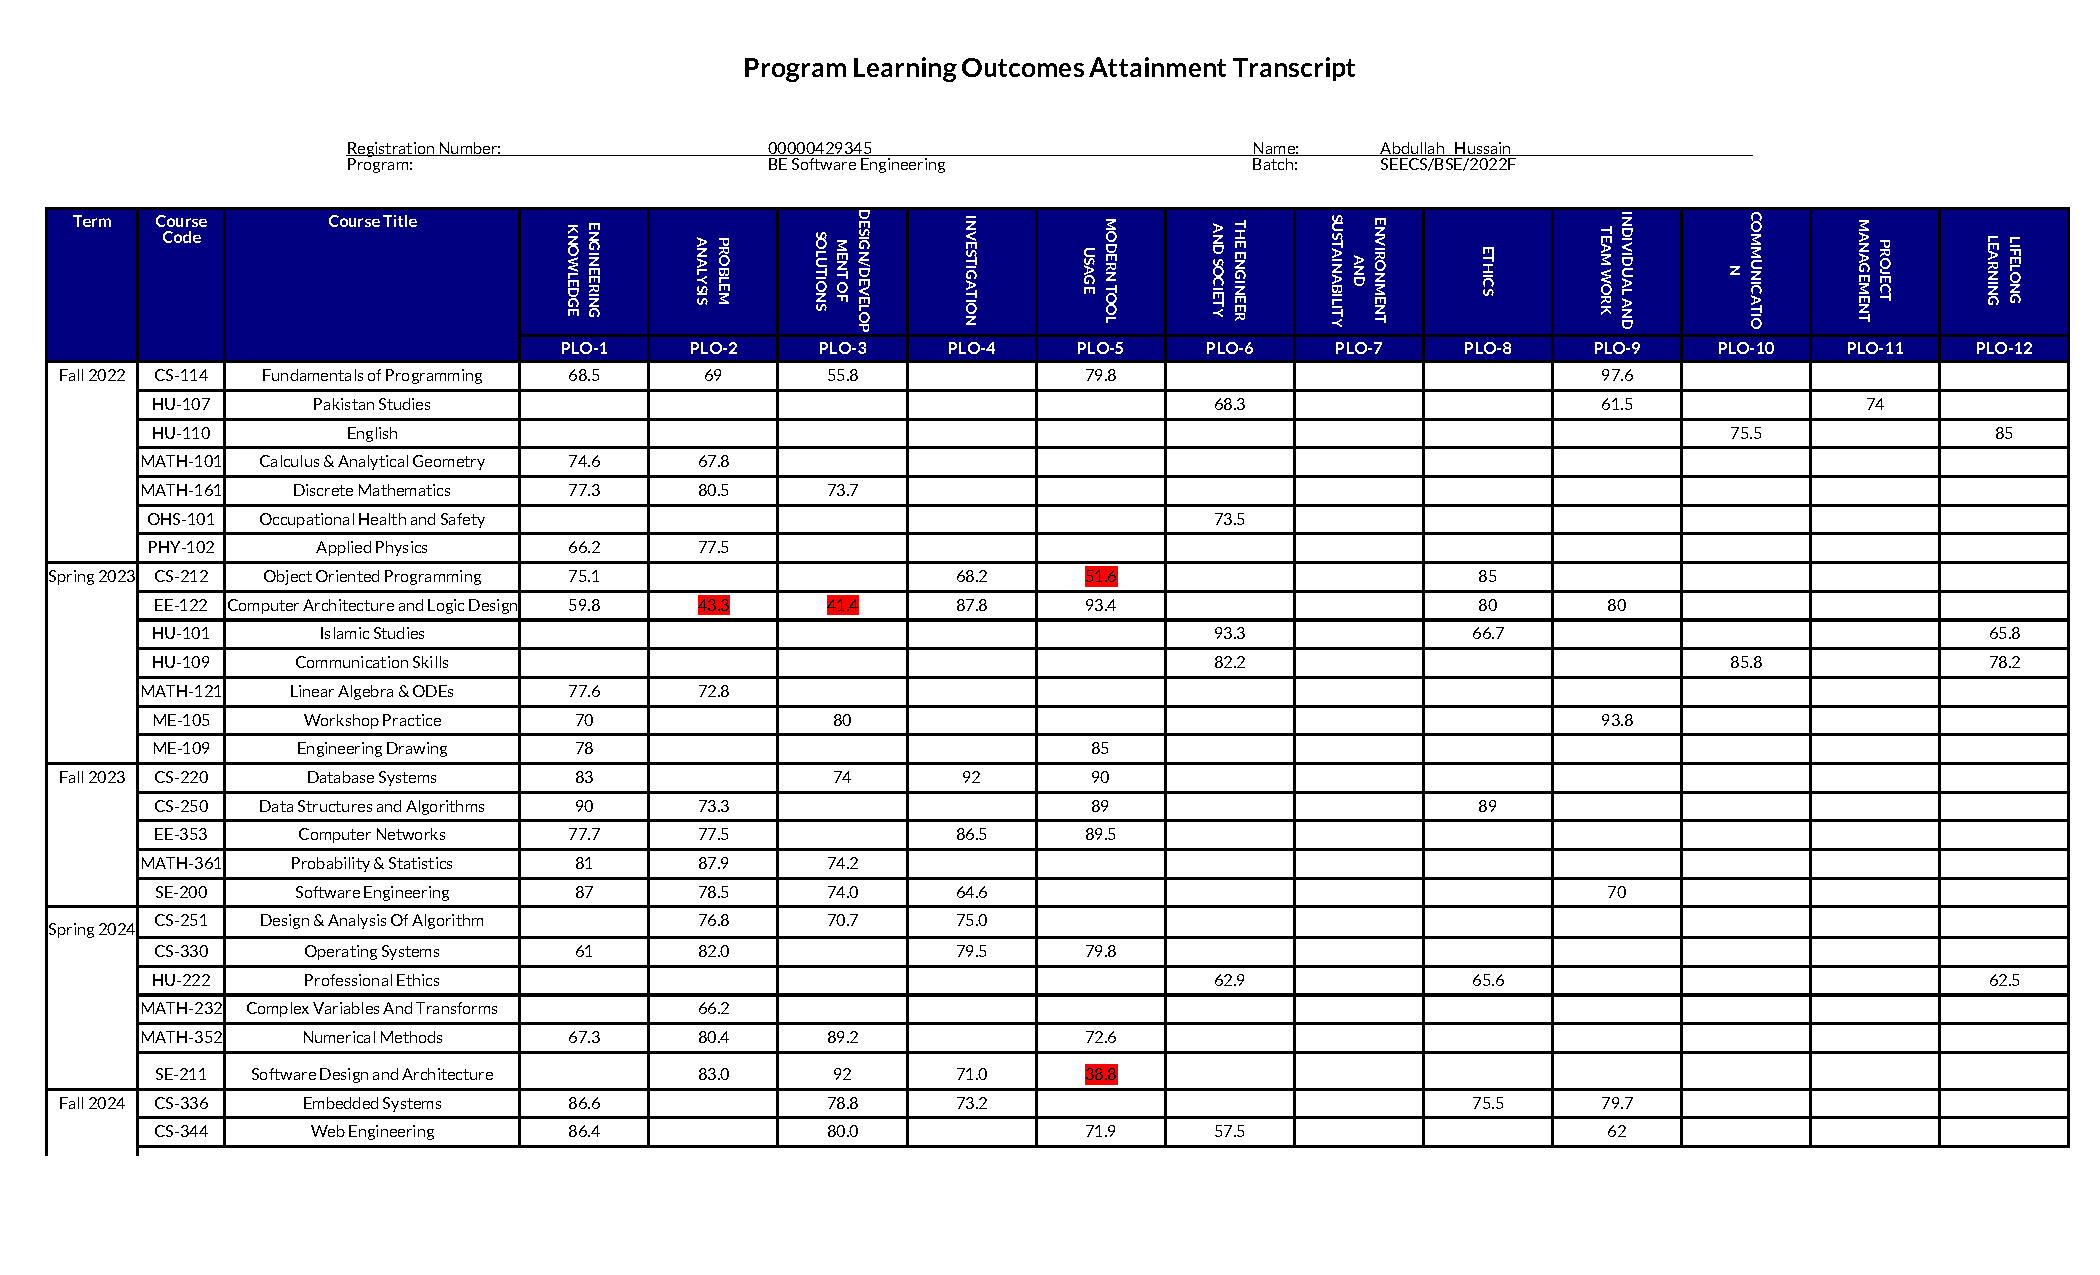
\includepdf[
  pages=1,
    landscape,
    scale=0.80,
  pagecommand={\thispagestyle{plain}%
    \noindent{\Large\bfseries\thesection\quad PLO Attainment Transcript}}
]{appendices/criterion_3/Annex-5-PLO-Attainment-Transcript.pdf}
\end{landscape}
% ---- Pages 2 to end: unchanged, at full size ----
\includepdf[
  pages={2-},
    landscape,
  pagecommand={\thispagestyle{plain}}%
]{appendices/criterion_3/Annex-5-PLO-Attainment-Transcript.pdf}


%\clearpage
%\section{Lab Rubric Based Evaluation}
\clearpage
\refstepcounter{section}
\phantomsection 
\label{app:criteria-3_Lab Rubric Based Evaluation}
\addcontentsline{toc}{section}{\protect\numberline{\thesection}Rubric Based Lab Evaluation}
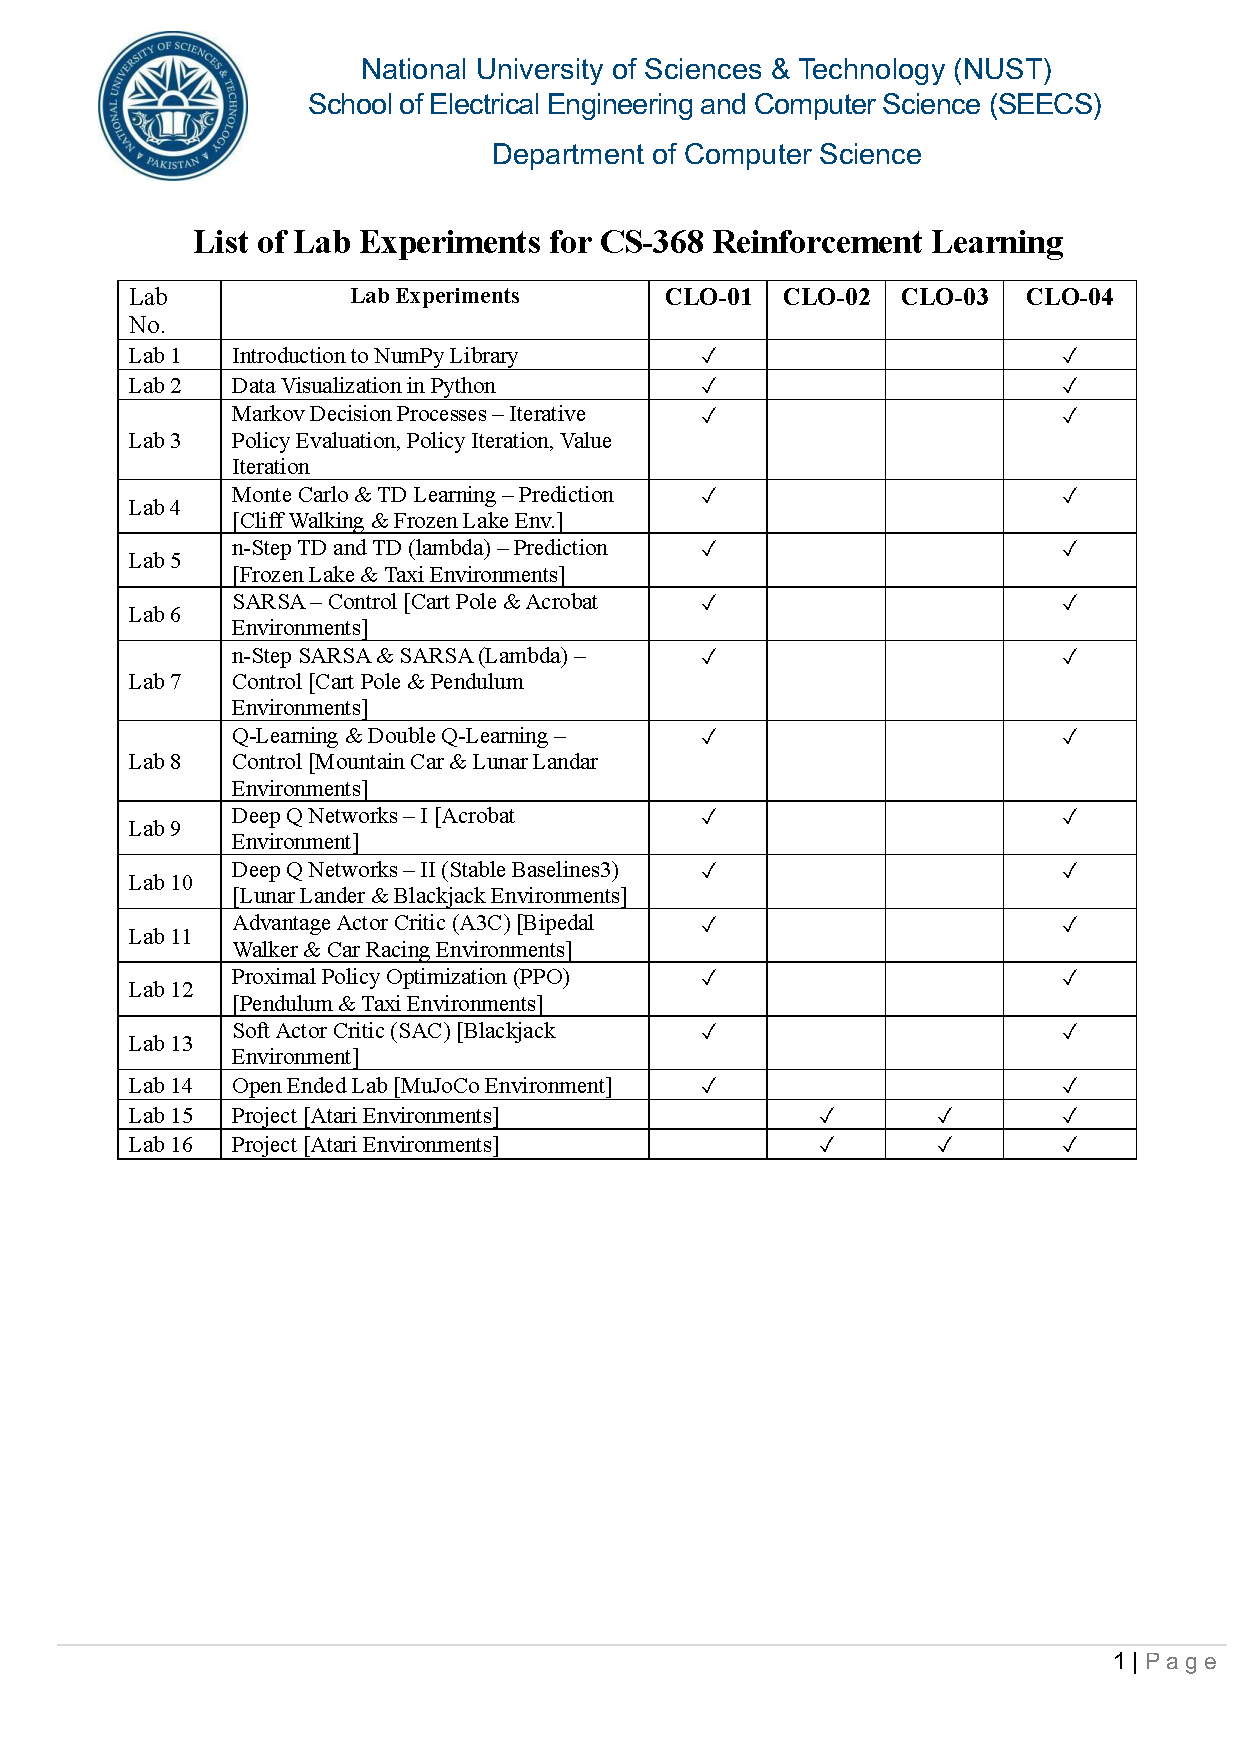
\includepdf[
  pages={1},
  scale=0.85,
  offset=0 -1.5cm,
  pagecommand={\thispagestyle{plain}%
    \noindent{\Large\bfseries\thesection\quad Rubric Based Lab Evaluation}}
]{appendices/criterion_3/Annex-6-Lab-Rubric Based Evaluation.pdf}

\includepdf[
  pages={2-},
  pagecommand={\thispagestyle{plain}}
]{appendices/criterion_3/Annex-6-Lab-Rubric Based Evaluation.pdf}

%\includefullannexure{appendices/criterion_3/Annex-6-Lab-Rubric Based Evaluation.pdf}


%\section{Sample Lab Manual}
\clearpage
\refstepcounter{section}
\phantomsection 
\label{app:criteria-3_Sample Lab Manual}
\addcontentsline{toc}{section}{\protect\numberline{\thesection}Sample Lab Manual}
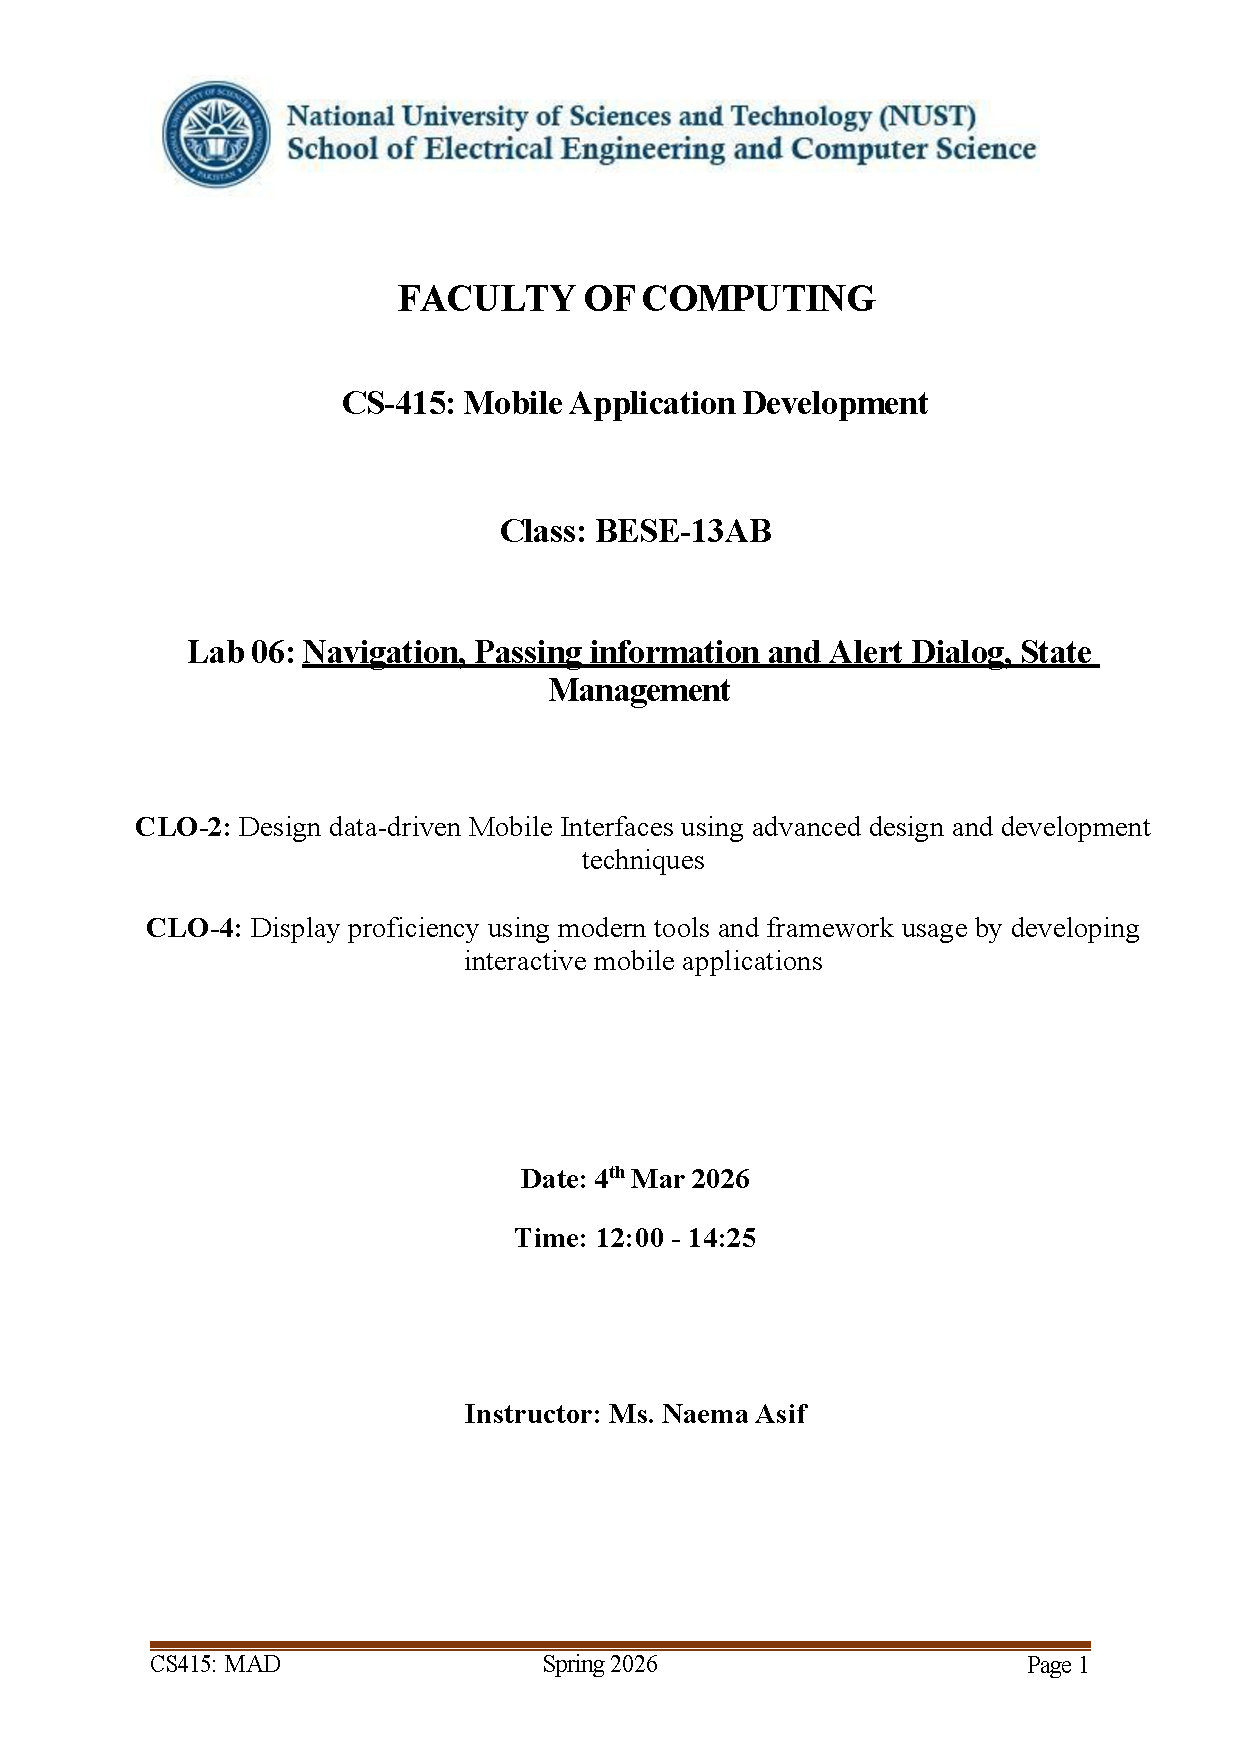
\includepdf[
  pages={1},
  scale=0.85,
  offset=0 -1.5cm,
  pagecommand={\thispagestyle{plain}%
    \noindent{\Large\bfseries\thesection\quad Sample Lab Manual}}
]{appendices/criterion_3/Annex-7-Sample-Lab-Manual.pdf}

\includepdf[
  pages={2-},
  pagecommand={\thispagestyle{plain}}
]{appendices/criterion_3/Annex-7-Sample-Lab-Manual.pdf}
%\includefullannexure{appendices/criterion_3/Annex-7-Sample-Lab-Manual.pdf}

%\clearpage
%\section{Sample Open Ended Lab}
%\label{app:criteria-3_Sample Open Ended Lab}
%\includefullannexure{appendices/criterion_3/Annex-8-Solving-MuJoCo-Environment-Using-RL-(Open-Ended-Lab).pdf}
\clearpage
\refstepcounter{section}
\phantomsection 
\label{app:criteria-3_Sample Open Ended Lab}
\addcontentsline{toc}{section}{\protect\numberline{\thesection}Sample Open Ended Lab}
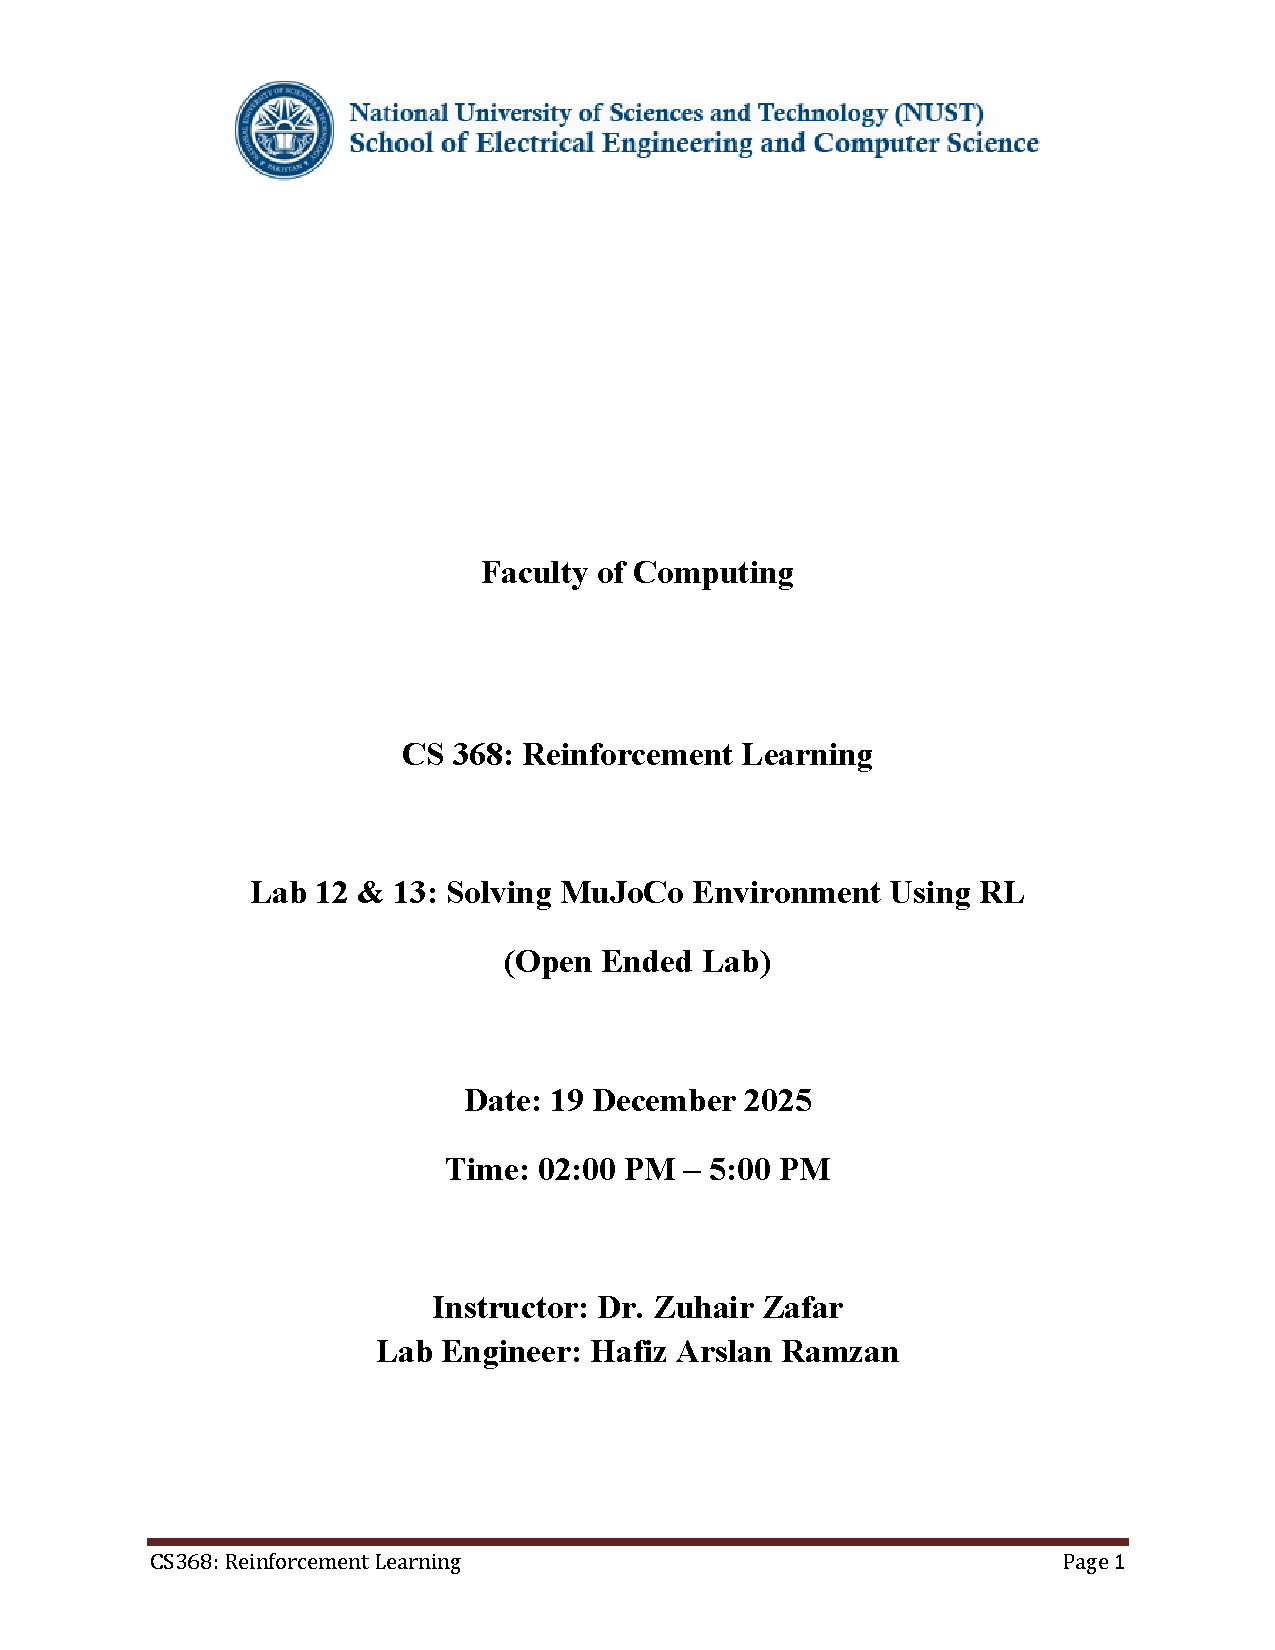
\includepdf[
  pages={1},
  scale=0.85,
  offset=0 -1.5cm,
  pagecommand={\thispagestyle{plain}%
    \noindent{\Large\bfseries\thesection\quad Sample Open Ended Lab}}
]{appendices/criterion_3/Annex-8-Solving-MuJoCo-Environment-Using-RL-(Open-Ended-Lab).pdf}

\includepdf[
  pages={2-},
  pagecommand={\thispagestyle{plain}}
]{appendices/criterion_3/Annex-8-Solving-MuJoCo-Environment-Using-RL-(Open-Ended-Lab).pdf}

\clearpage
%\section{System of Instruction and Examination}
%\includefullannexure{appendices/criterion_3/Annex-9-System-of-instructions-and-examination.pdf}

\refstepcounter{section}
\phantomsection 
\label{app:criteria-3_System of instruction and examination}
\addcontentsline{toc}{section}{\protect\numberline{\thesection}System of Instruction and Examination}
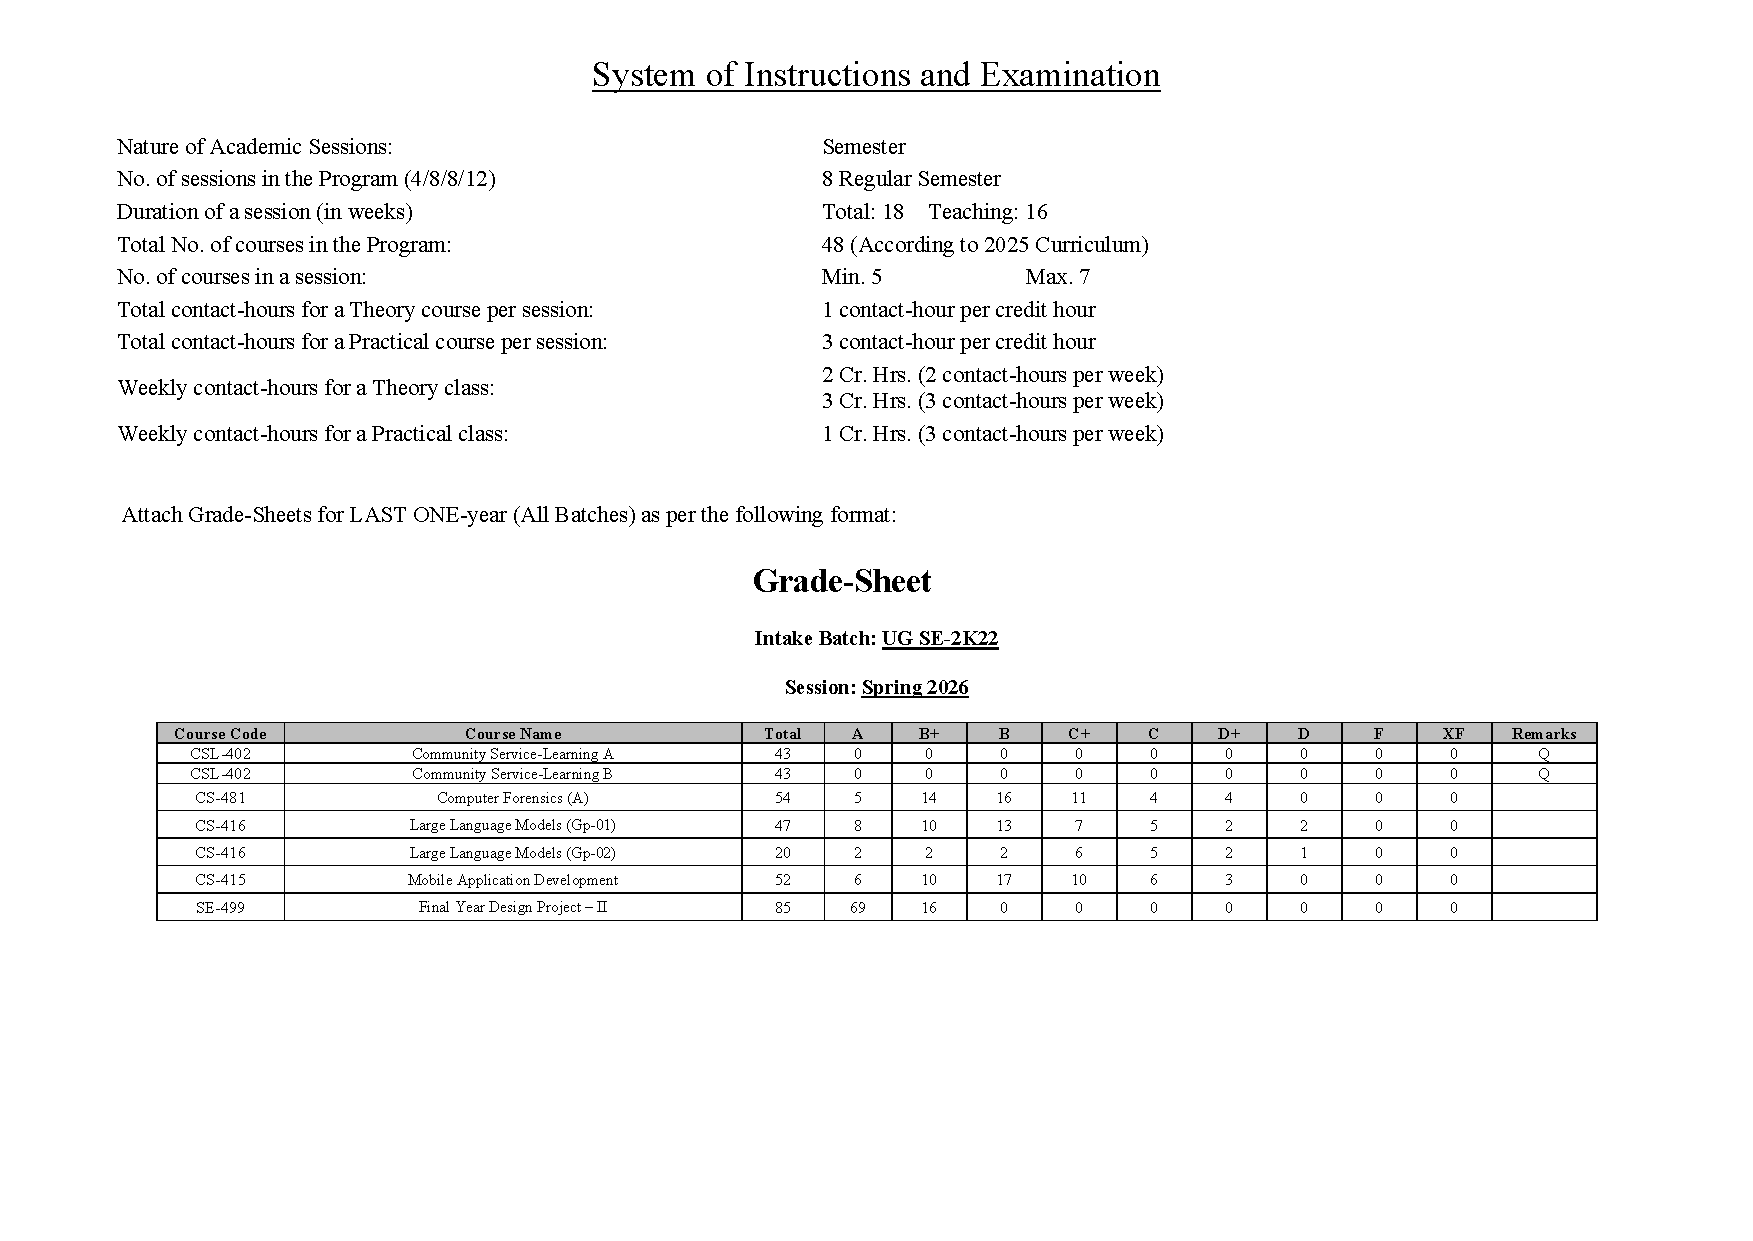
\includepdf[
  pages=1,
  landscape,
  scale=0.85,
  offset=1.5cm 0,
  pagecommand={\thispagestyle{plain}%
    \noindent\rotatebox{90}{\Large\bfseries\thesection\quad System of Instruction and Examination}}
]{appendices/criterion_3/Annex-9-System-of-instructions-and-examination.pdf}
    
\includepdf[
  pages=2-,
  landscape,
  pagecommand={\thispagestyle{plain}}
]{appendices/criterion_3/Annex-9-System-of-instructions-and-examination.pdf}

\clearpage
%\section{CEP Policy for BESE Program}
%\label{app:criteria-3_CEP Policy for BESE Department}
%\includefullannexure{appendices/criterion_3/Annex-10-Request-for-CEP-and-OEL-Formalization.pdf}

%\refstepcounter{section}
%\phantomsection 
%\label{app:criteria-3_CEP Policy for BESE Department}
%\addcontentsline{toc}{section}{\protect\numberline{\thesection}CEP Policy for BESE Program}
%\includepdf[
%  pages={-},
%  scale=0.85,
  %offset=0 -1.5cm,
%  pagecommand={\thispagestyle{plain}%
    %\noindent{\Large\bfseries\thesection\quad CEP Policy for BESE Program}}
%]{appendices/criterion_3/Annex-10-Request-%for-CEP-and-OEL-Formalization.pdf}

%\clearpage
%\section{CEP Policy for BESE Program}
%\label{app:criteria-3_CEP Policy for BESE Department}
%\includefullannexure{appendices/criterion_3/Annex-10-Request-for-CEP-and-OEL-Formalization.pdf}

\clearpage
%\section{CEP Example}
%\label{app:criteria-3_CEP Example}
%\includefullannexure{appendices/criterion_3/Annex-11-Sample-CEP.pdf}

\refstepcounter{section}
\phantomsection 
\label{app:criteria-3_CEP Example}
\addcontentsline{toc}{section}{\protect\numberline{\thesection}CEP Example}
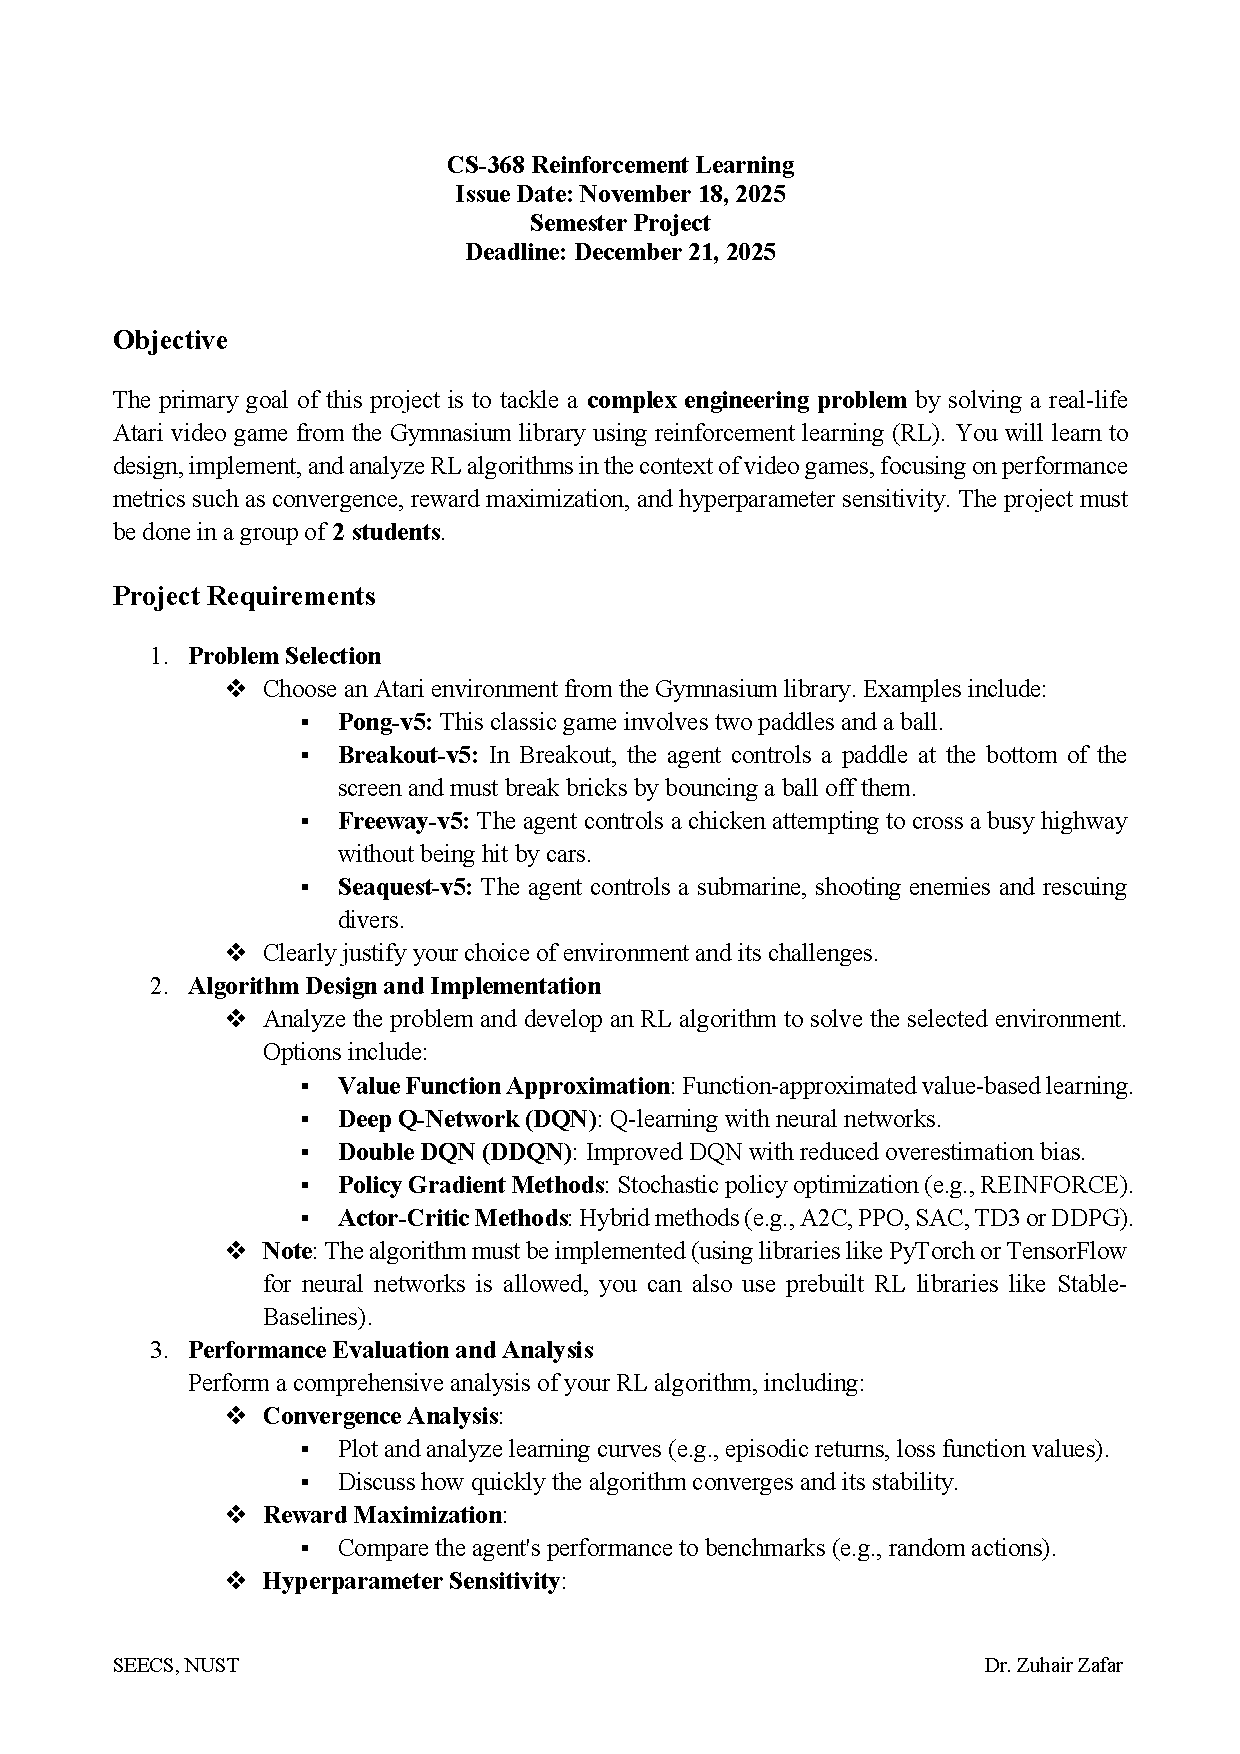
\includepdf[
  pages={1},
  scale=0.85,
  %offset=0 -1.5cm,
  pagecommand={\thispagestyle{plain}%
    \noindent{\Large\bfseries\thesection\quad CEP Example}}
]{appendices/criterion_3/Annex-11-Sample-CEP.pdf}
\includepdf[
  pages=2-,
  %landscape,
  pagecommand={\thispagestyle{plain}}
]{appendices/criterion_3/Annex-11-Sample-CEP.pdf}

\clearpage
\refstepcounter{section}
\phantomsection 
\label{app:criteria-3_FYP_Guidelines}
\addcontentsline{toc}{section}{\protect\numberline{\thesection}FYP Guidelines}
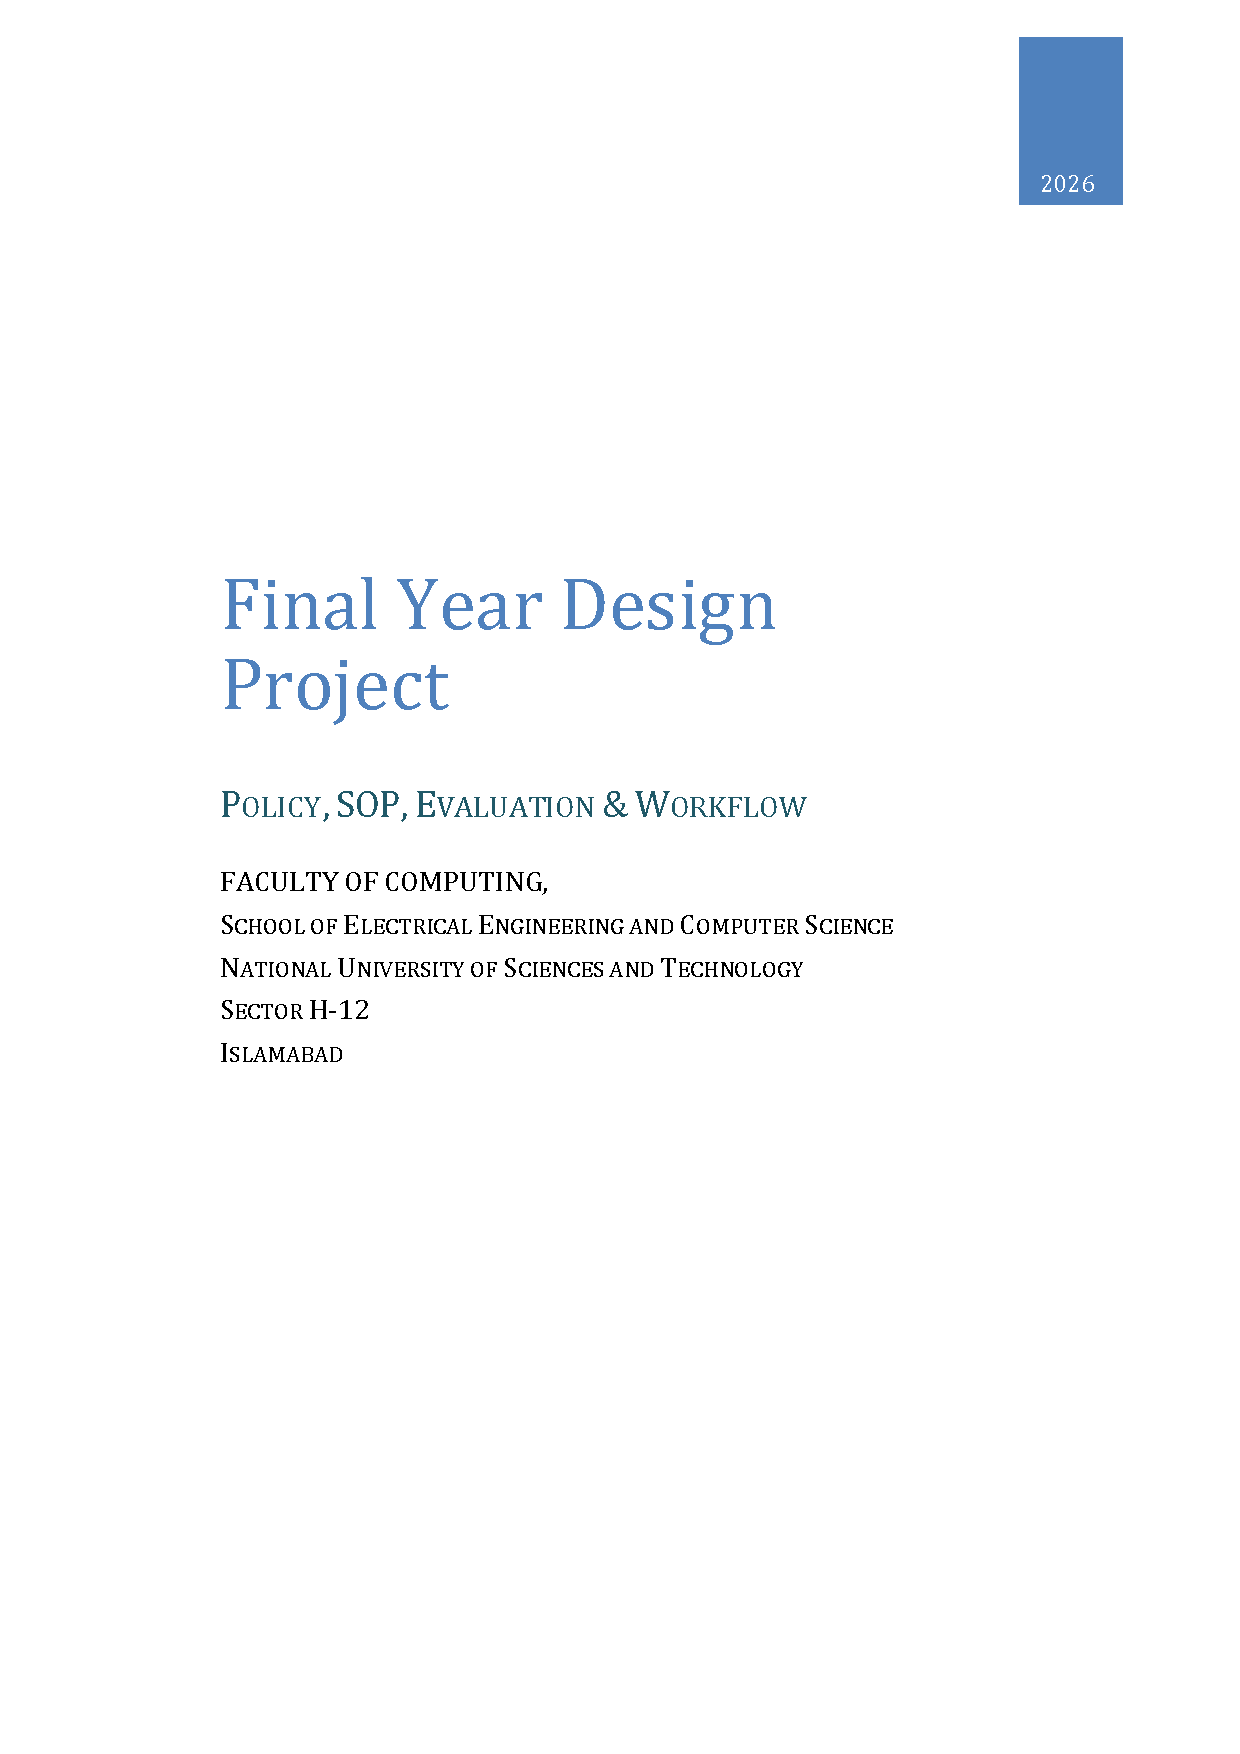
\includepdf[
  pages={1},
  scale=0.85,
  %offset=0 -1.5cm,
  pagecommand={\thispagestyle{plain}%
    \noindent{\Large\bfseries\thesection\quad FYP Guidelines}}
]{appendices/criterion_3/FYDP-SoP-Policy-2026.pdf}
\includepdf[
  pages=2-,
  %landscape,
  pagecommand={\thispagestyle{plain}}
]{appendices/criterion_3/FYDP-SoP-Policy-2026.pdf}

%\section{FYP Guidelines}

%\includefullannexure{appendices/criterion_3/FYDP-SoP-Policy-2026.pdf}

\clearpage
%\section{List of FYDP BESE 2K22 Batch}

%\includefullannexure{appendices/criterion_3/Annex-13-List_FYDP_BESE_2K22.pdf}

\refstepcounter{section}
\phantomsection 
\label{app:criteria-3_List of FYDP BESE 2K22 Batch}
\addcontentsline{toc}{section}{\protect\numberline{\thesection}List of FYDP BESE 2K22 Batch}
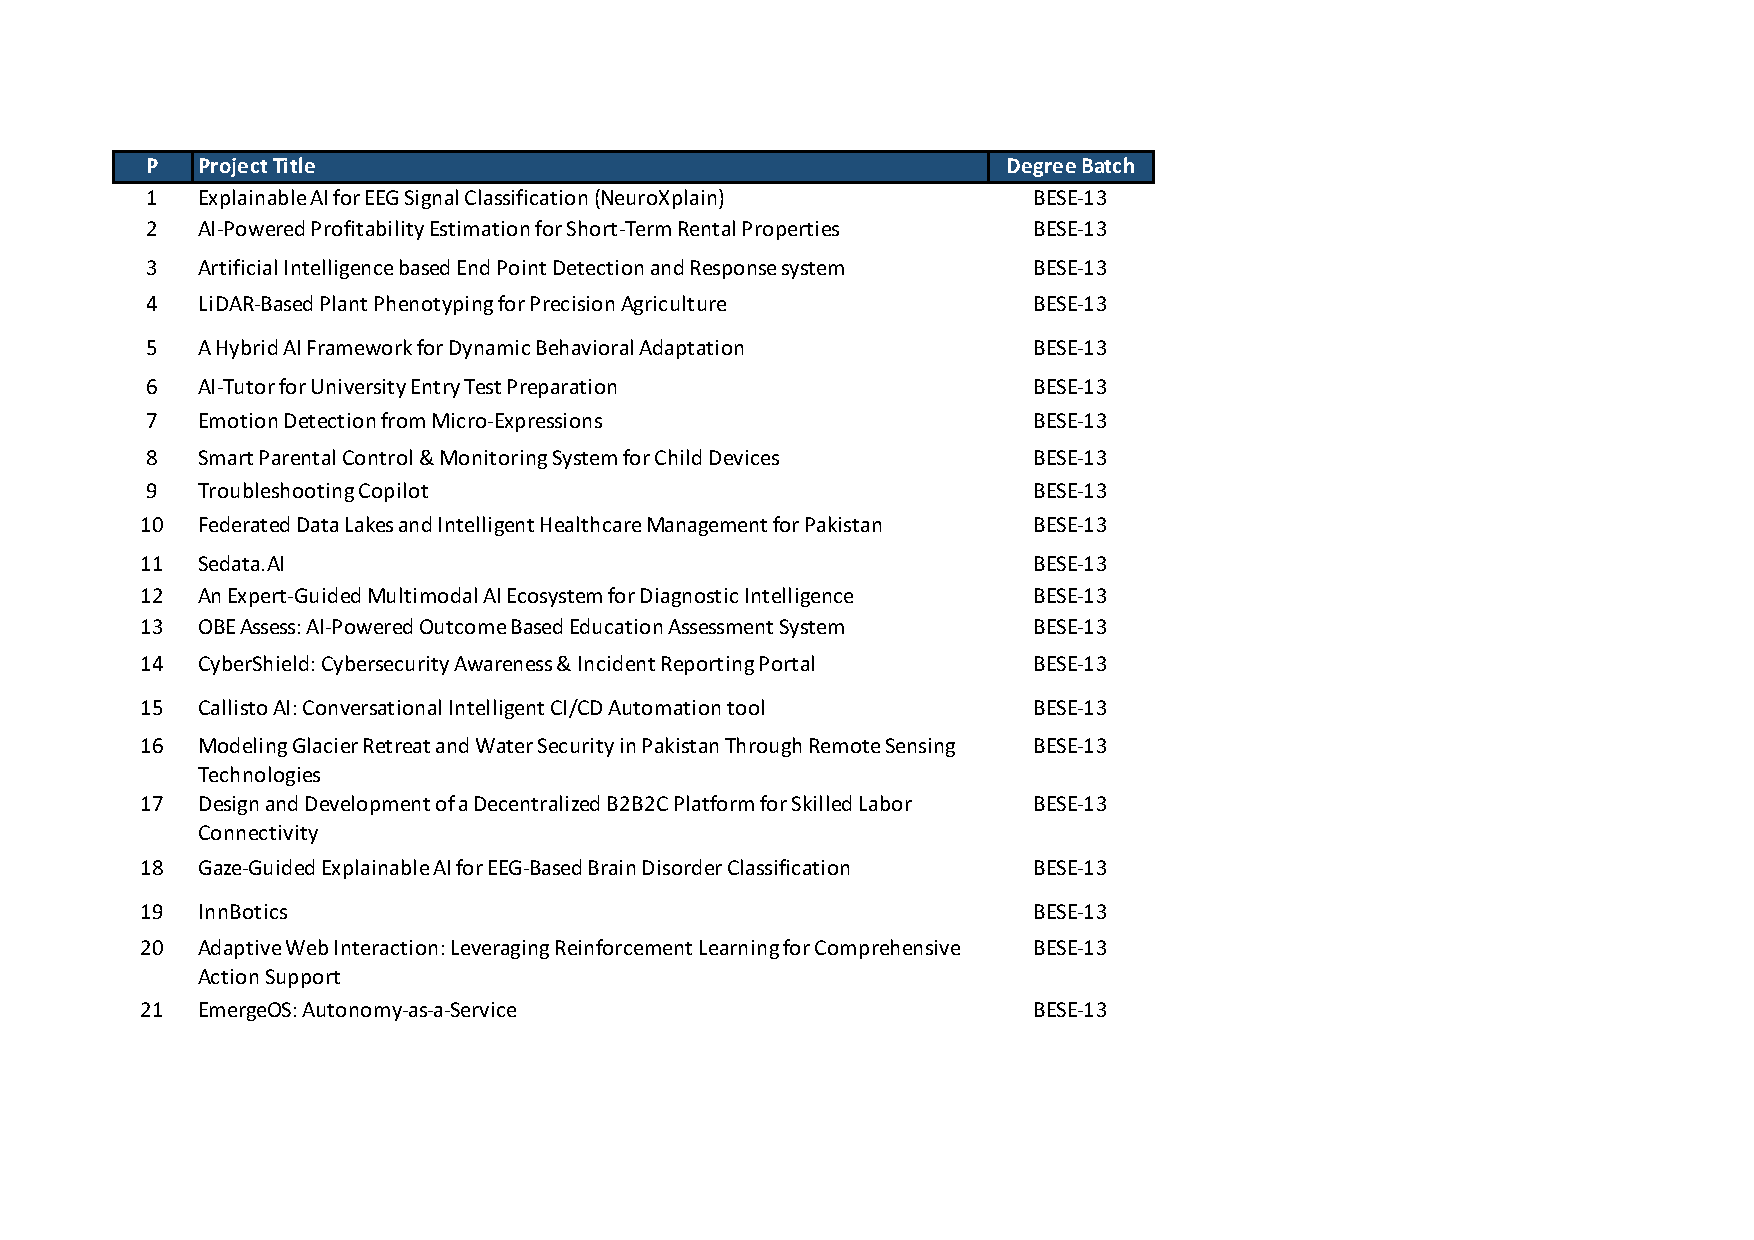
\includepdf[
  pages=1,
  scale=0.85,
  landscape,
  offset=0 -1.5cm,
  pagecommand={\thispagestyle{plain}%
    \noindent{\Large\bfseries\thesection\quad List of FYDP BESE 2K22 Batch}}
]{appendices/criterion_3/fydp-list-2k22.pdf}
    
\includepdf[
  pages=2-,
  landscape,
  pagecommand={\thispagestyle{plain}}
]{appendices/criterion_3/fydp-list-2k22.pdf}

%\clearpage
%\section{Sample Course Outline}
%\label{BSample Course Outline}
%\includefullannexure{appendices/criterion_2/CS-251 Design and Analysis of Algorithms Spring 2026.pdf}

